\subsection{センサノードの参加・離脱時の振る舞い}
いくつかのセンサノードが,グループへ参加・離脱する際の手法を述べる.\\ \\
前者について下記にシーケンス図\ref{fig:group_on_join}を示す.

\begin{enumerate}
    \item 新規センサノードがグループに参加するため,参加するグループを決定する必要がある.GLノードはデータ集約時以外は,Adv Packetに自身のBLEサービスUUIDを載せAdvを行う.
    \item 新規センサノードは,起動時にBLEスキャンを実行し周囲に参加可能なグループがあるか探索する.
    \item 発見した場合は,そのグループに参加し,そうでない場合はLoRaWANで直接センサデータを送信する.
\end{enumerate}

後者について,下記にシーケンス図\ref{fig:group_on_leave}を示す.

\begin{enumerate}
    \item ノードが故障や電池切れで離脱する場合は,NSがデバイスを管理しているので,N回通信が来なかった場合に,グループリストからセンサノードを取り除く.
    \item GLノードの次回通信時に,更新したグループリストを通知する.
\end{enumerate}

\begin{figure}[]
    \begin{center}
    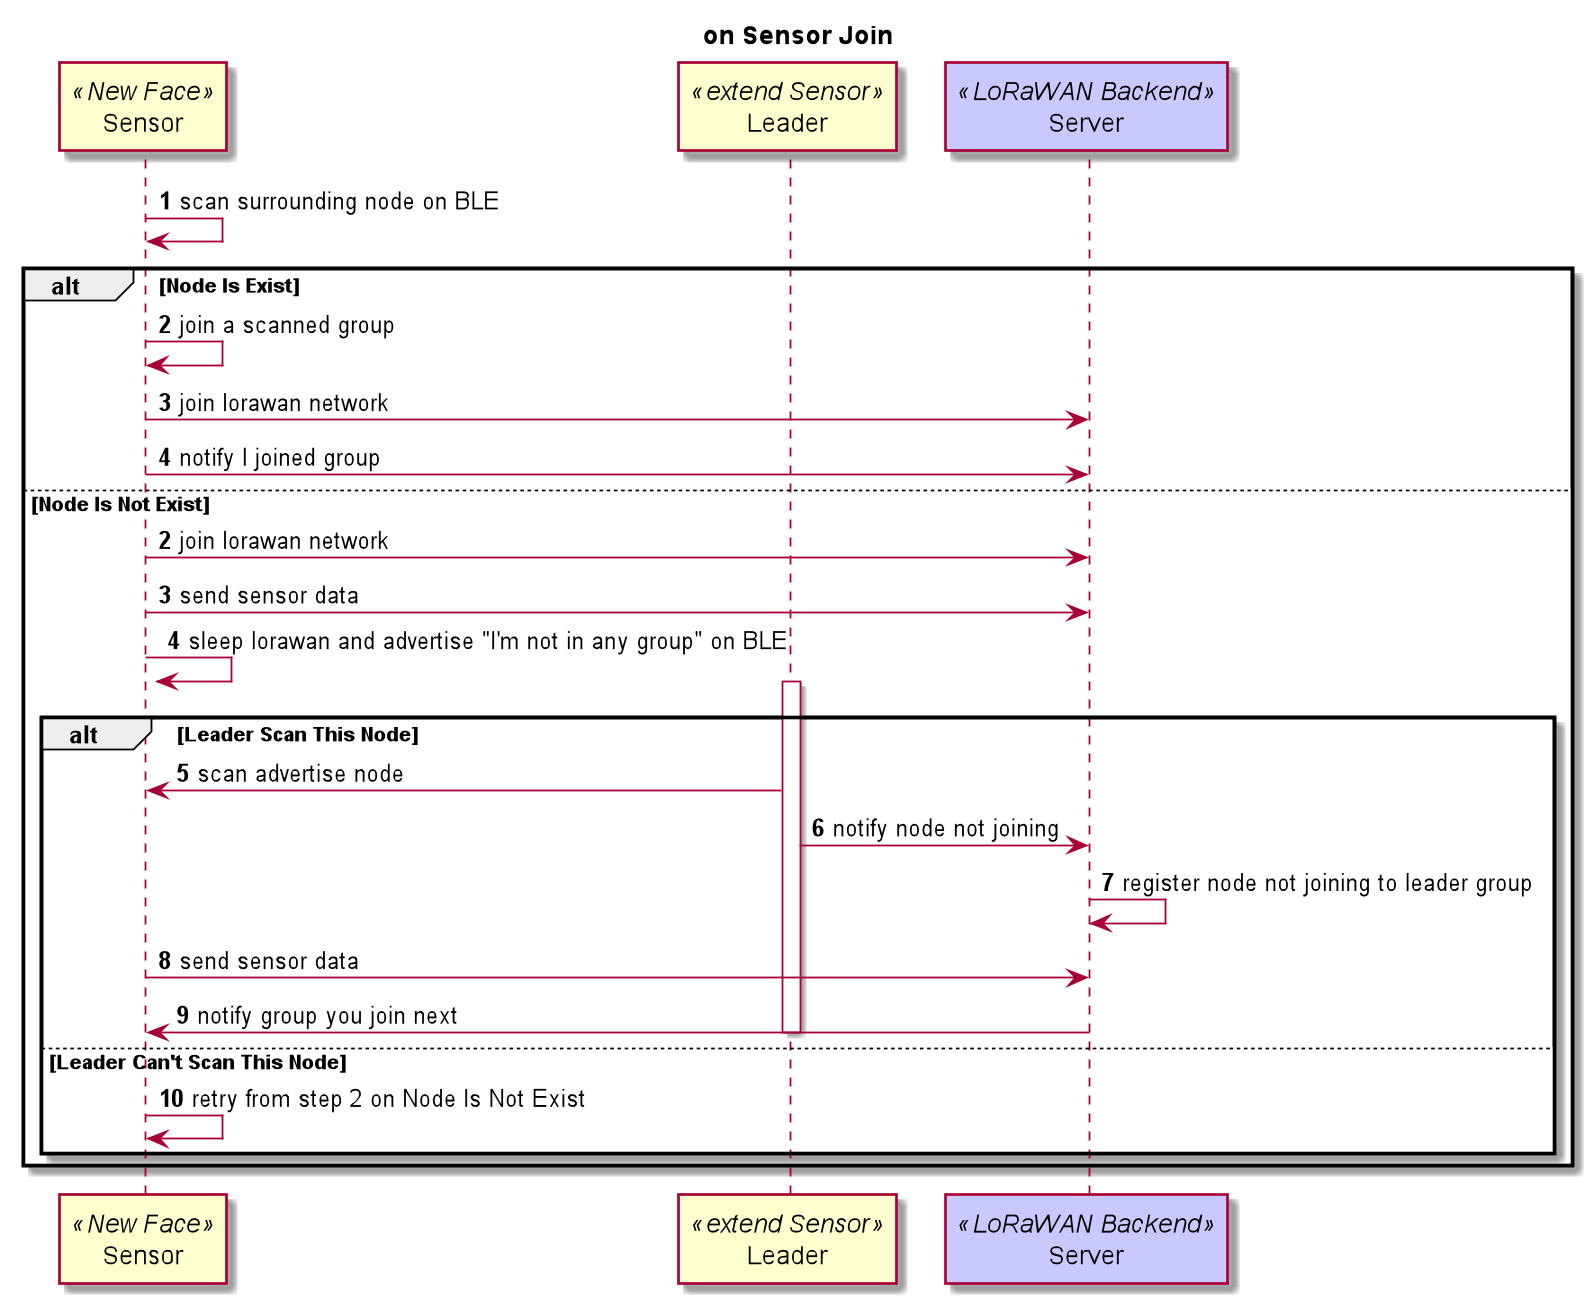
\includegraphics[width=14cm]{figures/グループ化_ネットワーク参加時.png}
    \caption{ネットワーク参加時の振る舞い}
    \label{fig:group_on_join}
    \end{center}
\end{figure}


\begin{figure}[]
    \begin{center}
    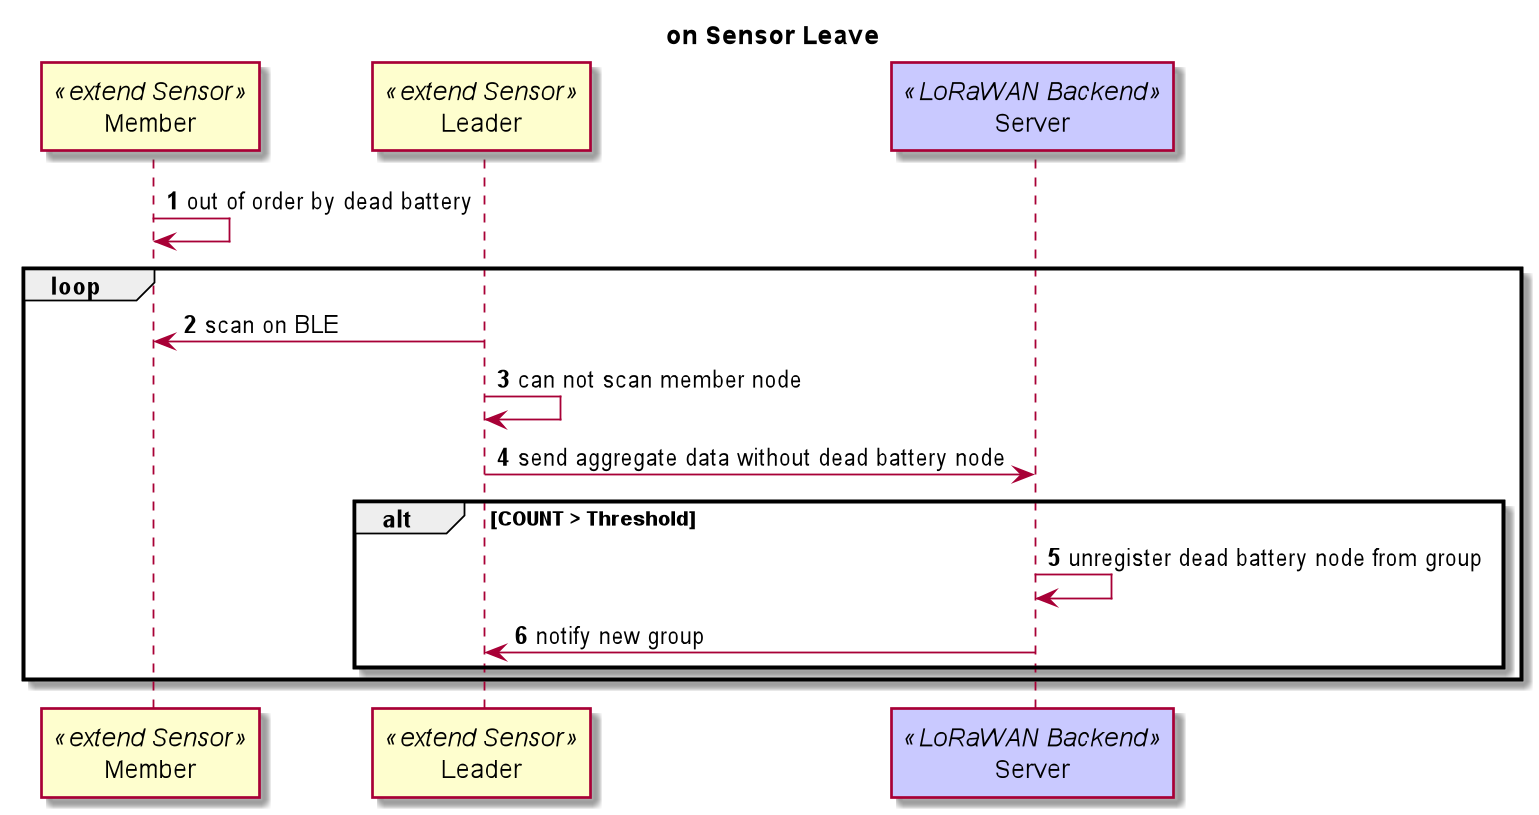
\includegraphics[width=14cm]{figures/グループ化_ネットワーク離脱時.png}
    \caption{ネットワーク離脱時の振る舞い}
    \label{fig:group_on_leave}
    \end{center}
\end{figure}